% GAME_HARD_01_PRESENTATION_INTRODUCTION.tex
\section{Introduction}

% GRAPHICS VERIFICATION
\subsection{Graphics Verification}
\begin{frame}
\frametitle{GRAPHICS VERIFICATION}

\begin{figure}[ht]
  \begin{minipage}[b]{0.3\linewidth}
    \centering
    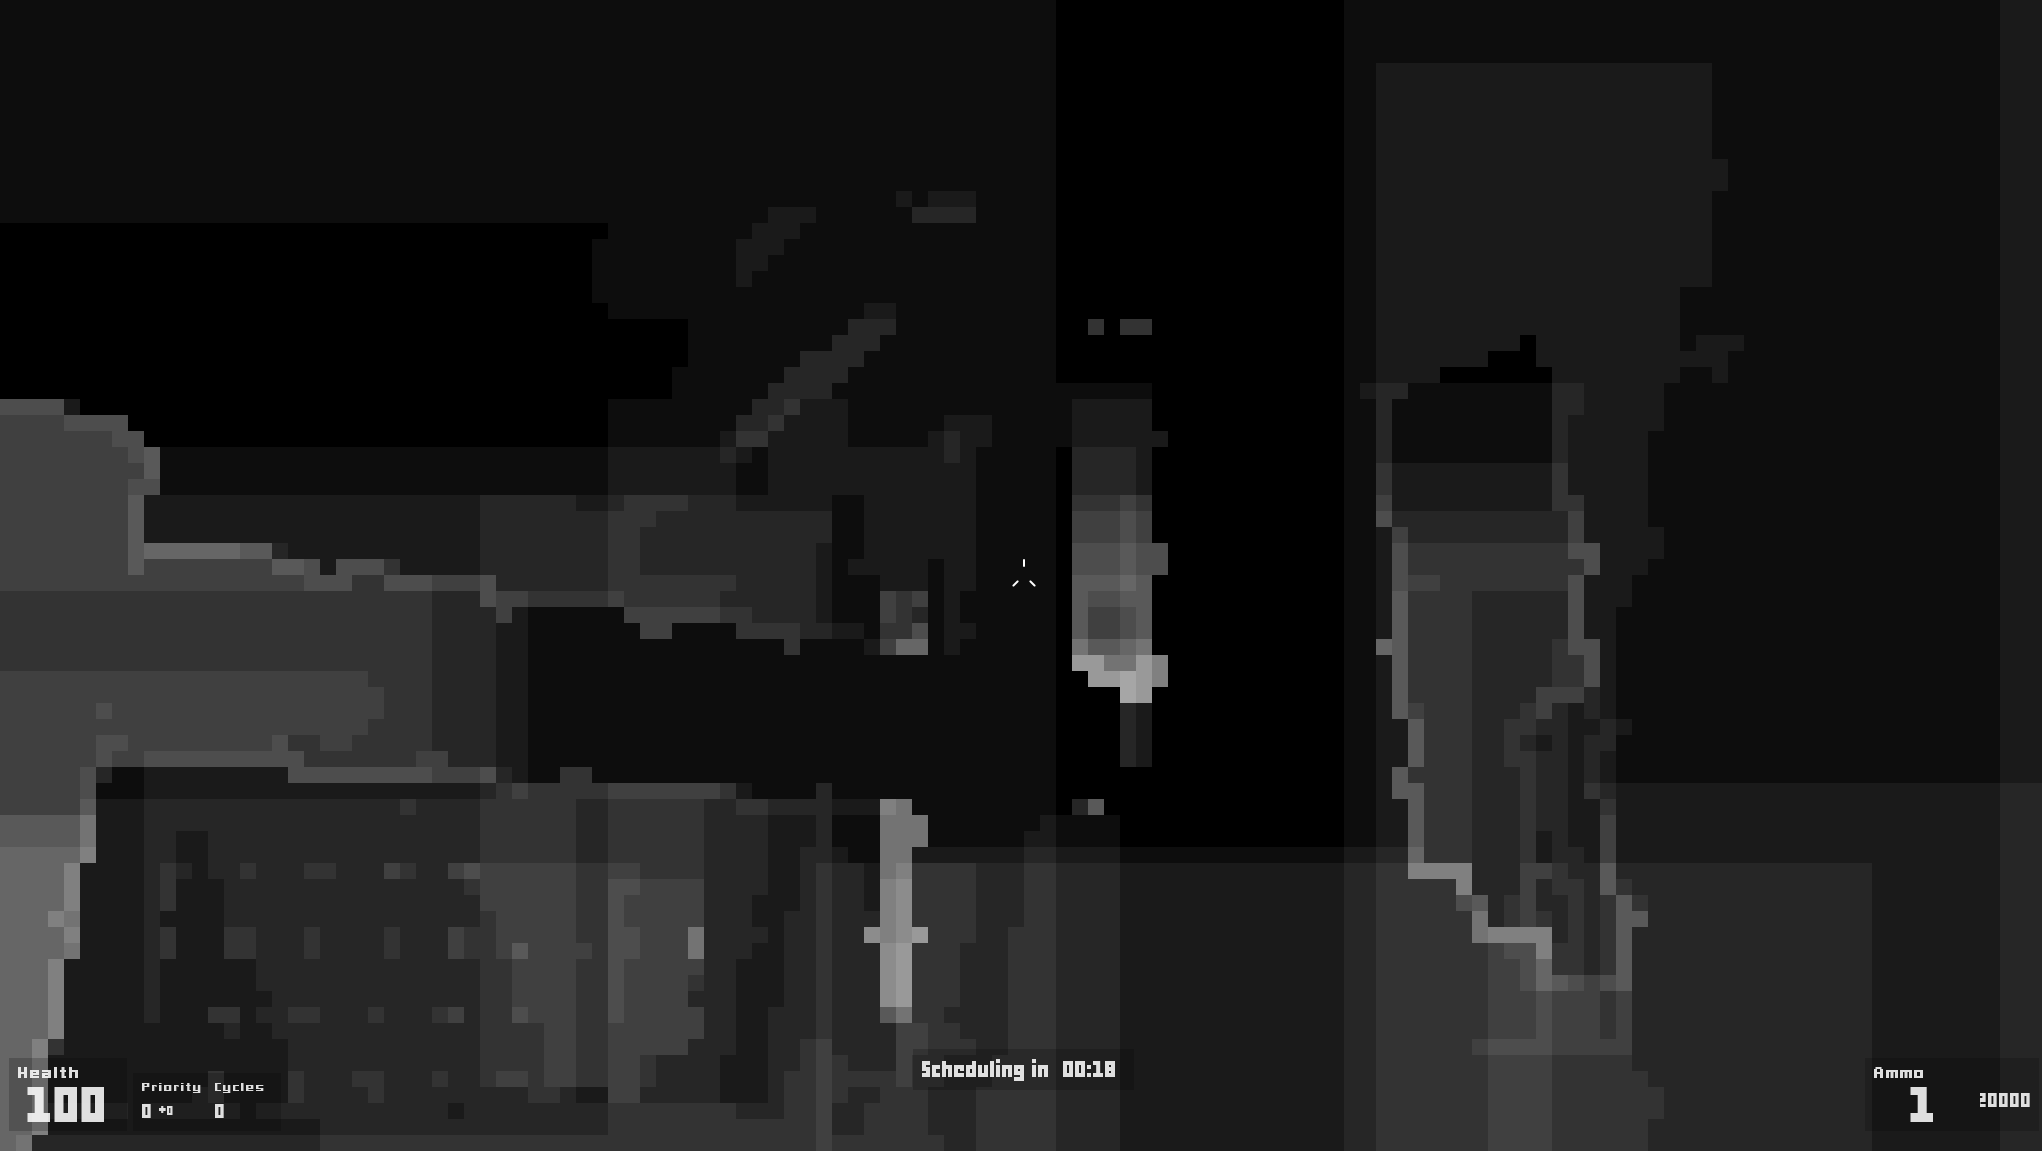
\includegraphics[width=1.0\textwidth]{img/tbds1.png}
  \end{minipage}
  \hspace{0.25cm}
  \begin{minipage}[b]{0.3\linewidth}
    \centering
    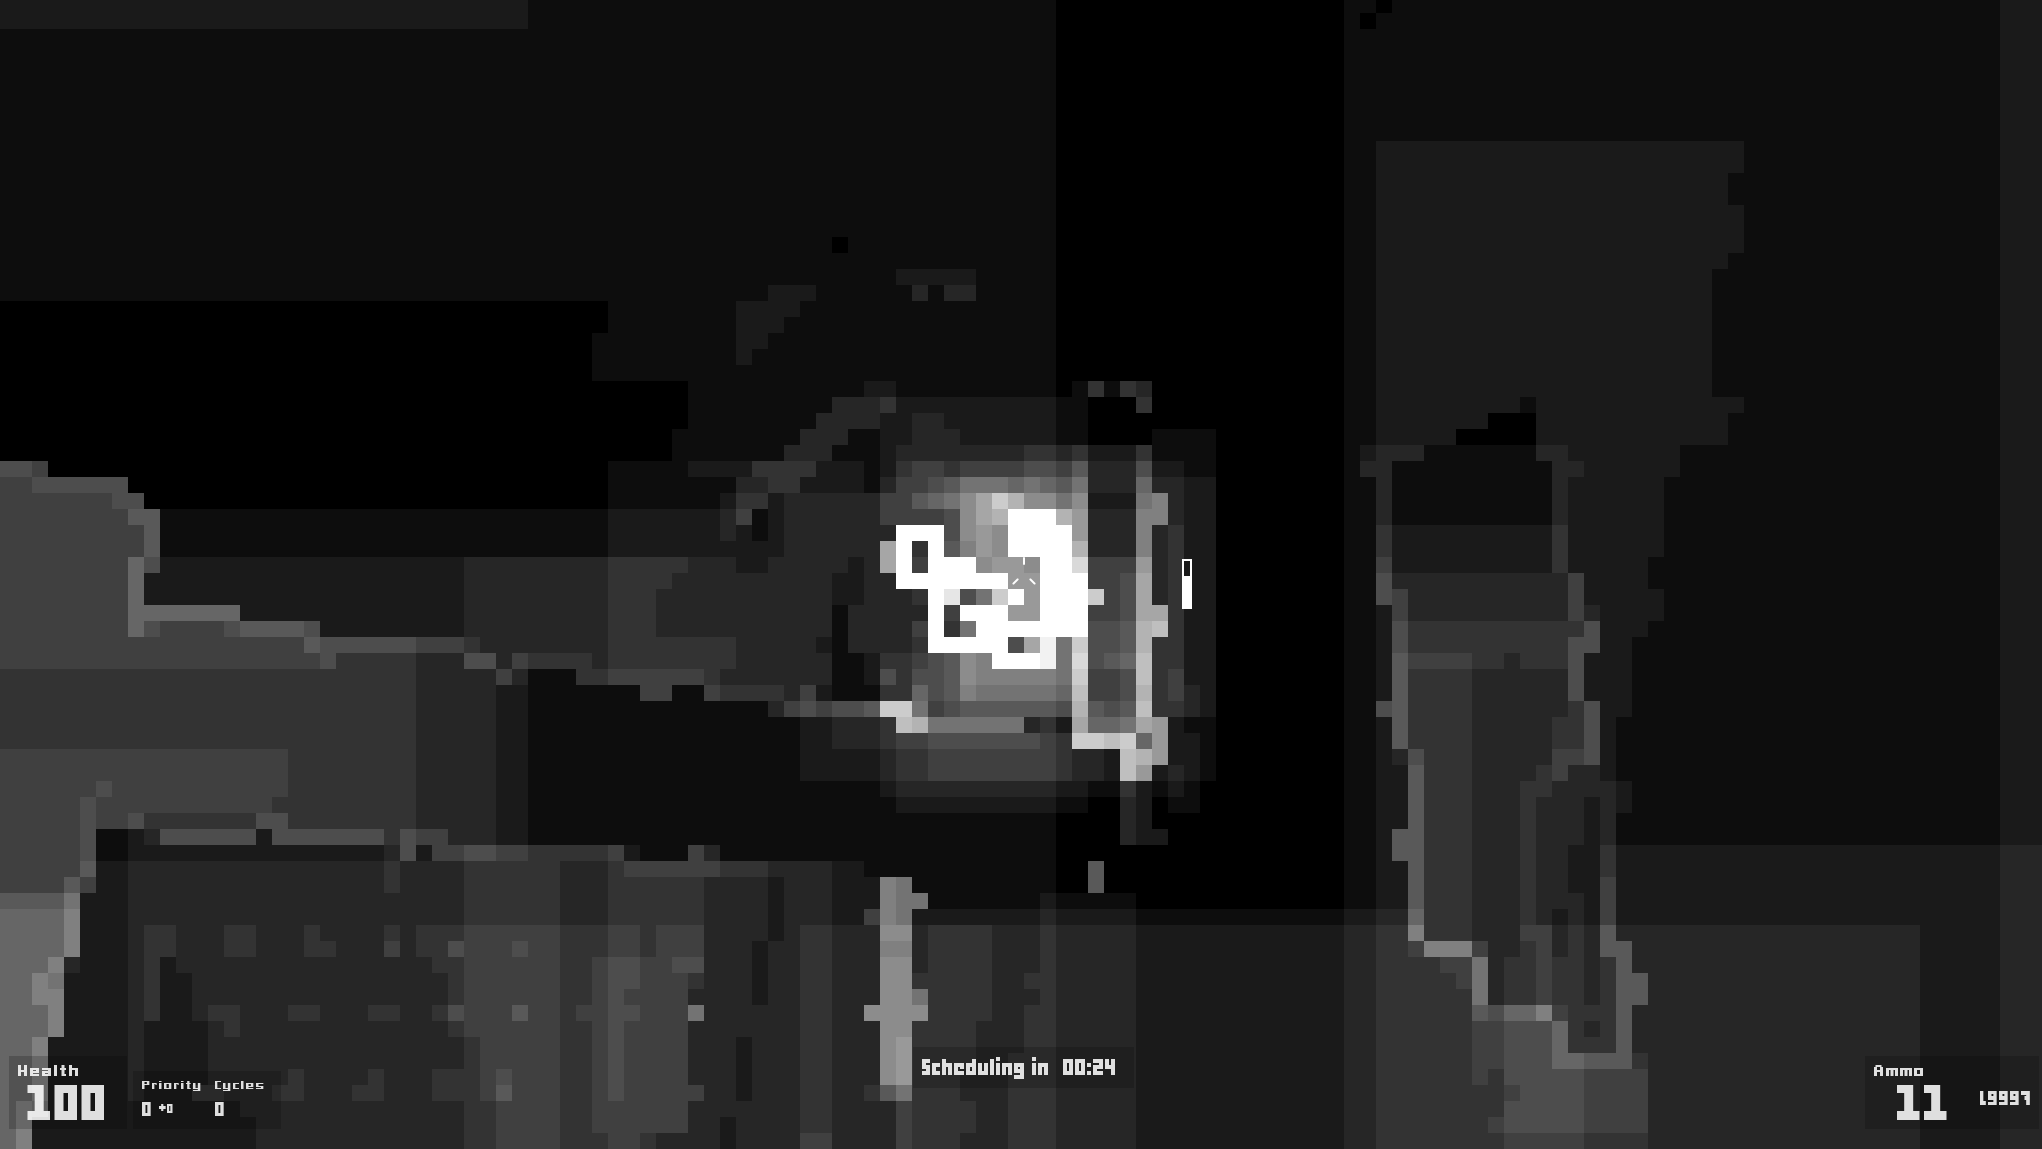
\includegraphics[width=1.0\textwidth]{img/tbds2.png}
  \end{minipage}
  \hspace{0.25cm}
  \begin{minipage}[b]{0.3\linewidth}
    \centering
    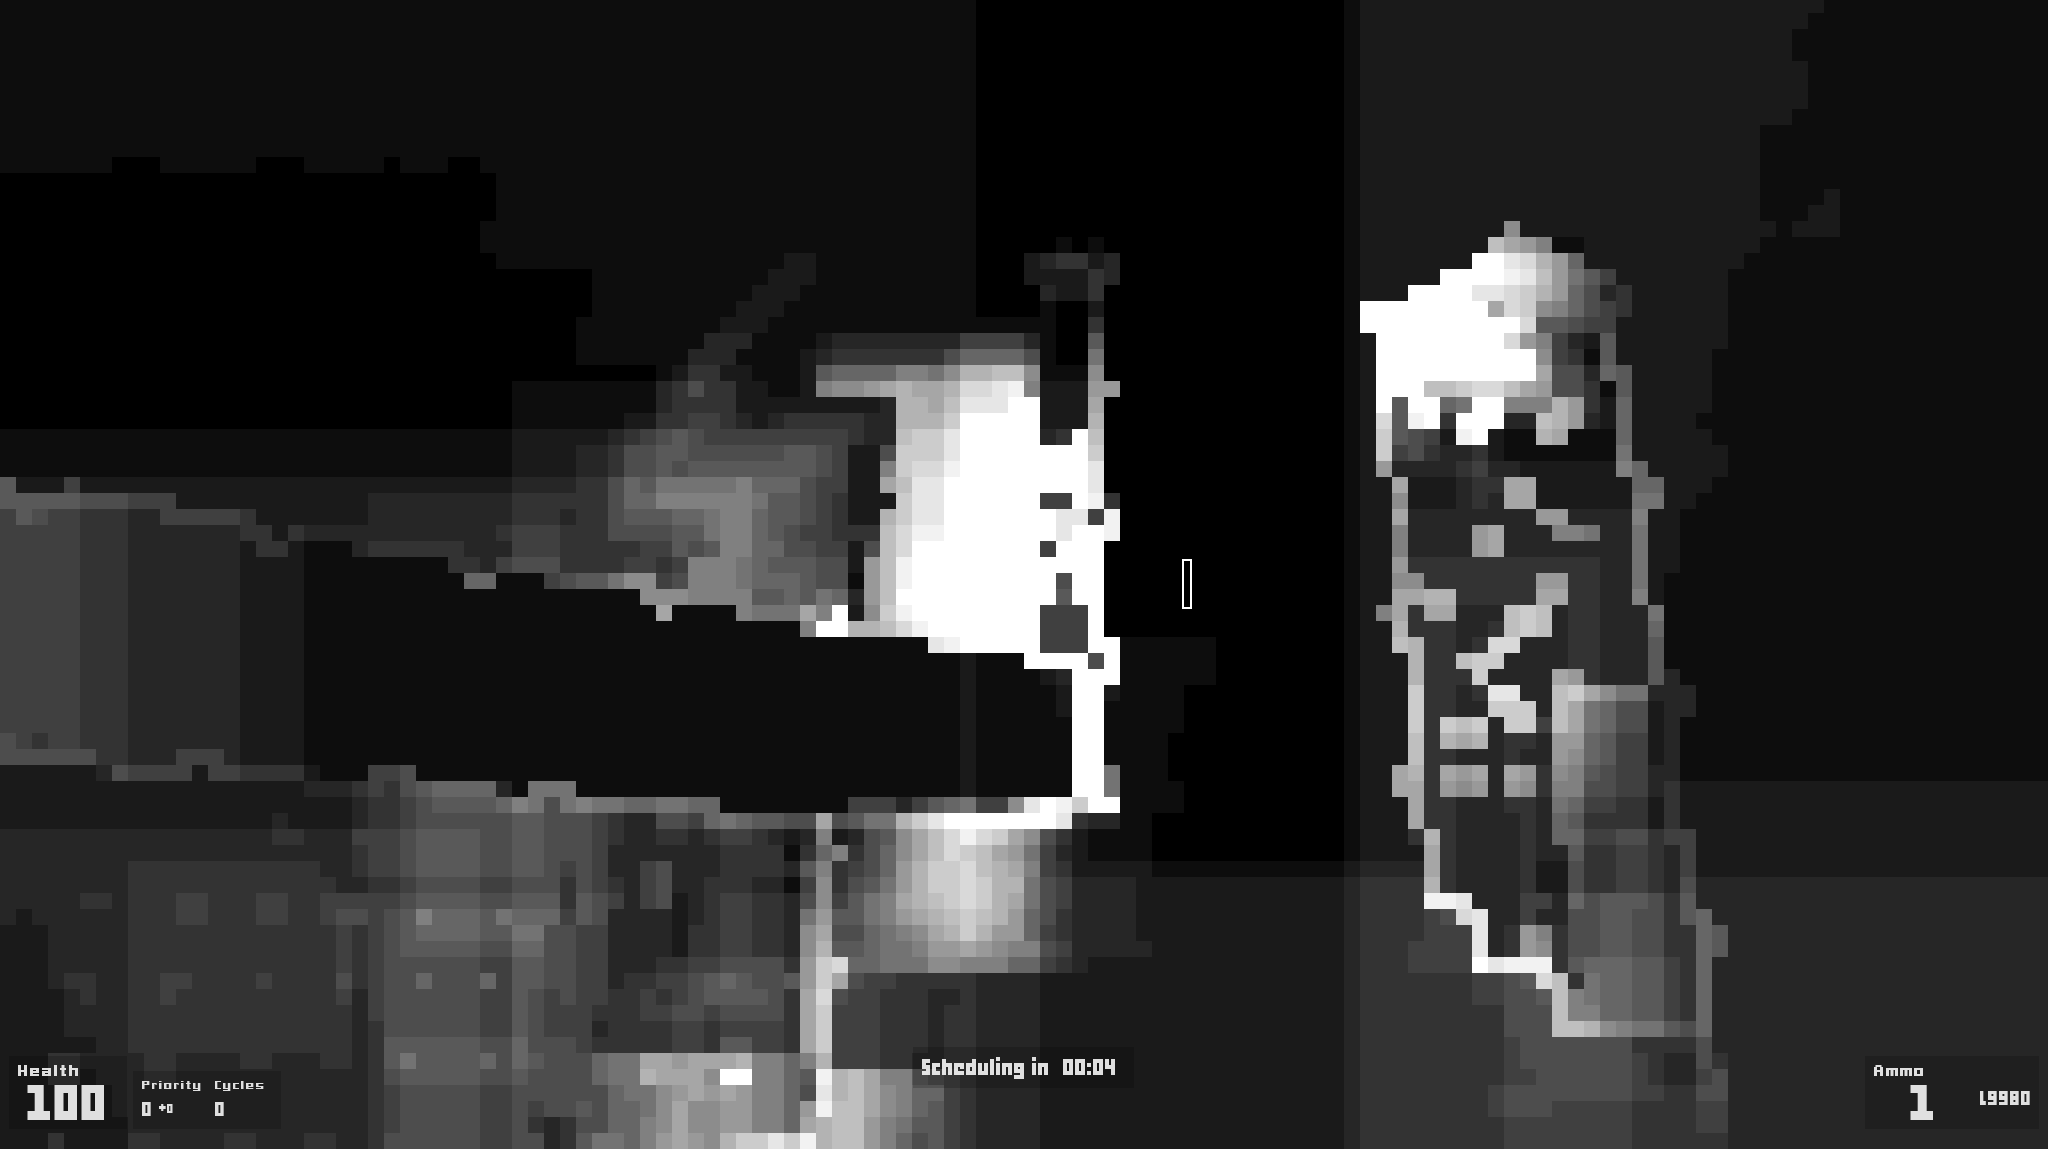
\includegraphics[width=1.0\textwidth]{img/tbds3.png}
  \end{minipage}
  \label{fig:tilingvisualization}
  \caption{\href{https://github.com/L0mion/xkill-source}{%
      Tile-based deferred shading using DirectCompute.}}
\end{figure}

\begin{figure}[ht]
  \begin{minipage}[b]{0.3\linewidth}
    \centering
    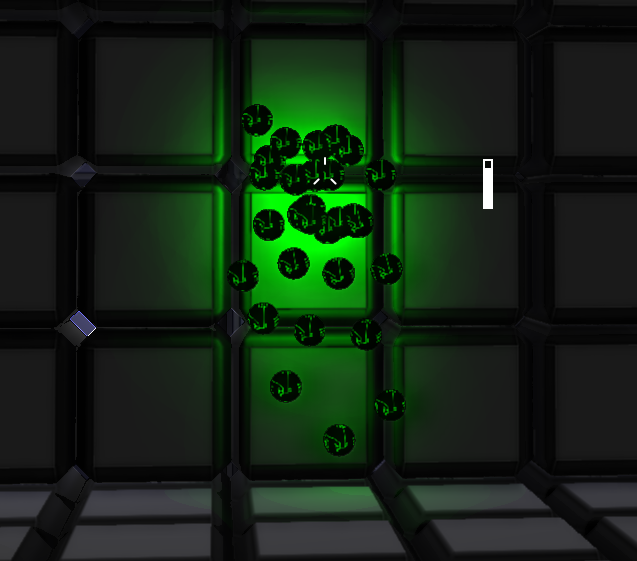
\includegraphics[width=1.0\textwidth]{img/tbds.png}
    \caption{AMD\textit{*≠}}
  \end{minipage}
  \hspace{0.25cm}
  \begin{minipage}[b]{0.3\linewidth}
    \centering
    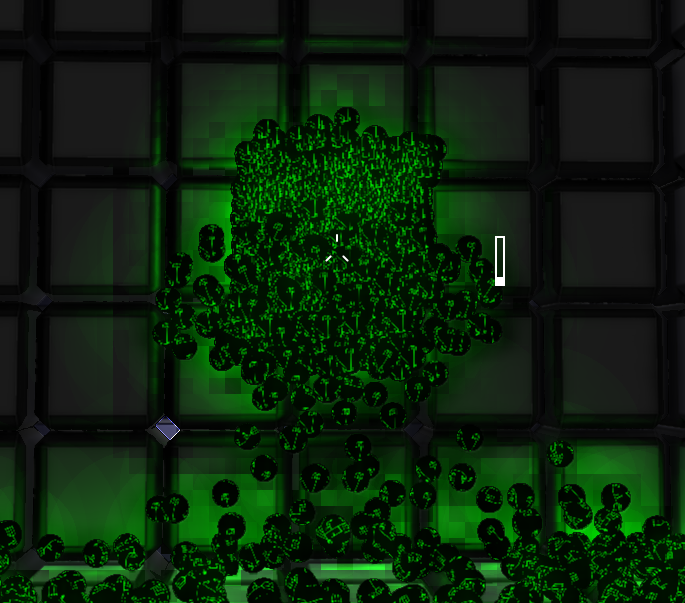
\includegraphics[width=1.0\textwidth]{img/tbds_error.png}
    \caption{NVIDIA\textit{*≠}}
  \end{minipage}
  \label{fig:tilingerror}
\end{figure}

\end{frame}

% THE REFERENCE DEVICE DRIVER
\subsection{The Reference Device Driver}
\begin{frame}
\frametitle{THE REFERENCE DEVICE DRIVER}

The Reference Device Driver or Reference Rasterizer:
\begin{itemize}
\item Shipped with the DirectX SDK
\item \textbf{Not} included in Windows run-times
\item Intended for debugging purposes:
  \begin{itemize}
  \item Feature testing
  \item Demonstration purposes
  \end{itemize}
\item Does feature some native instruction optimization, but all-in-all not intended for retail applications
\end{itemize}

\end{frame}

% GRAPHICS SIMULATION
\subsection{Graphics Simulation}
\begin{frame}
\frametitle{GRAPHICS SIMULATION}

\begin{itemize}
\item Common method of verifying GPU workloads, such as computer graphics, by eliminating dependency to third-party drivers and hardware
\item May also practical for the purposes of extracting additional debugging or profiling data
\item Sometimes a necessity on platforms lacking conformant hardware
\item Often orders of magnitude too slow for complex applications
\end{itemize}

\end{frame}

% MICROSOFT WARP
\subsection{Microsoft WARP}
\begin{frame}
\frametitle{MICROSOFT WARP}

\href{http://msdn.microsoft.com/en-us/library/windows/desktop/gg615082(v=vs.85)%
  .aspx}{'...a high speed, fully conformant software rasterizer...':}
\begin{itemize}
\item Introduced in Direct3D 11
\item Derived from the Reference Device Driver
\item Included in Windows 7 and 8 runtimes
\end{itemize}

Optimized for CPU execution using:
\begin{itemize}
\item Thread pooling for modern multicore CPUs
\item Batch execution (possibly similar in concept to NVIDIA warps)
\item JIT compilation:
  \begin{itemize}
  \item SSE2 and SSE4.1 SIMD
  \item x86 native instructions
  \end{itemize}
\end{itemize}

See also: \href{http://www.mesa3d.org/llvmpipe.html}{the Gallium llvmpipe driver}

\end{frame}
